
\documentclass[10pt]{article} 
\usepackage[final]{graphicx} 
\usepackage{amsfonts} 
 \usepackage{amsmath}

\topmargin-.5in 
\textwidth6.6in 
\textheight9in 
\oddsidemargin0in 
 
\def\ds{\displaystyle} 
\def\d{\partial} 

 
\begin{document} 

%%SUBSECTION OF SYSTEM DYNAMICS

\section{System Dynamics}

 The governing equations of the system dynamics described on Section \ref{sec:methods} are the following: \\

\begin{eqnarray} 
\label{SDeqn}
\frac{dS}{dt} = - \frac{\beta_{I}SI+\beta_{H}SH+\beta_{F}SF}{N}\\
\frac{dE}{dt} =  \frac{\beta_{I}SI+\beta_{H}SH+\beta_{F}SF}{N}-\alpha E\\
\frac{dI}{dt} =  \alpha E - [\gamma_{H}\theta + \gamma_{I}(1-\theta)(1-\delta_{1})+\gamma_{D}(1-\theta)\delta_{1}]I\\
\frac{dH}{dt} = \gamma_{H}\theta I - [\gamma_{DH}\delta_{2}+\gamma_{IH}(1-\delta_{2})]H\\
\frac{dF}{dt} = \gamma_{D}(1-\theta) \delta_{1} I + \gamma_{DH}\delta_{2} H-\gamma_{F} F\\
\frac{dR}{dt} = \gamma_{I}(1-\theta)(1- \delta_{1}) I + \gamma_{IH}(1-\delta_{2}) H-\gamma_{F} F
\end{eqnarray}\\

\noindent where each of the parameters are defined on Table \ref{tab:parameters} \\


%INSIGHT MAKER DESCRIPTION AND RESULTS
\subsection{Insight Maker}
 Insight Maker is a powerful online tool used to model and simulate utilizing different approaches, such as System Dynamics, Agent-Based Modeling and imperative programming. Insight Maker allows to construct a graphical model interface to forecast the system response \cite{FortmannRoe}. We used InsightMaker platform to prototype our model and simulate stepping forward through time. More details about the platform and its functionality can be found in Fortmann-Roe's review \cite{FortmannRoe}. The platform uses fourth order Runge-Kutta differential equation solver for the system dynamics model and  first order Euler approximation for the Agent-Based model.

\noindent The implemented Insight Maker SD model is depicted in Figure \ref{fig:SD_IM} .


\begin{figure}[!h]
  \centering
  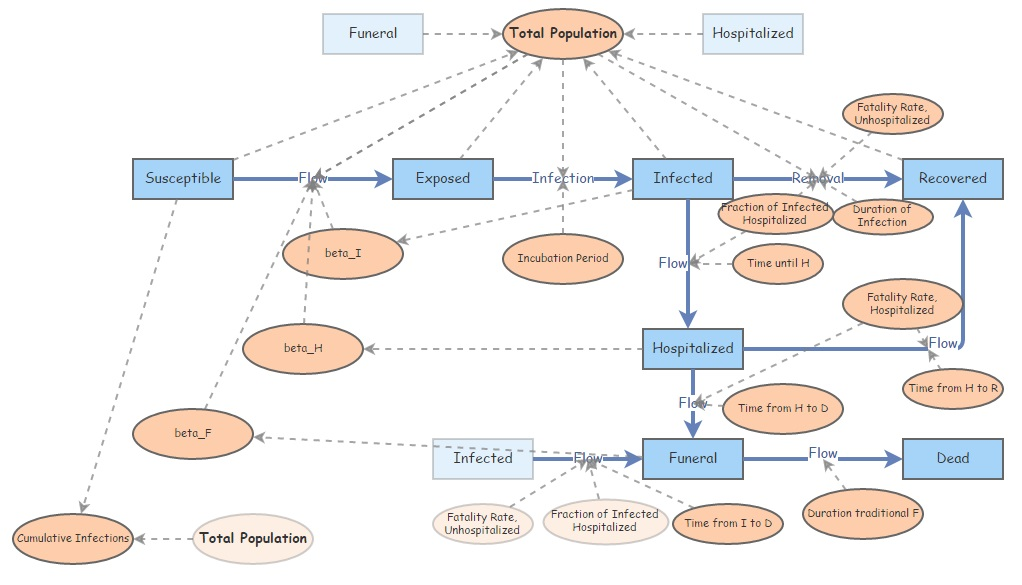
\includegraphics[width=0.7\textwidth]{SD_IM}
  \caption{ \bf Compartment model of the system dynamics implemented on Insight Maker}
\label{fig:SD_IM} 
\end{figure}\\

\noindent A normalized population fraction was simulated. The compartment S was initialized with a value of 999.999/1.000.000, and the compartment I with 1/1.000.000, meaning that there is an infected individual per every million of habitants, the rest of the compartments were set as 0. The flow between the compartments is specified in Figure \ref{fig:compartment.} and all the other parameters were initialized as shown in Table \ref{tab:parameters}.  As mention in Section \ref{sec:calibration}, the parameters were calibrated in two stages, before and after the international intervention. According with the time frame proposed, the change on the parameters was also implemented on Insight Maker. The links to the online models can be found on \cite{IM_AI} and  \cite{IM_BI}.  \\


% RESULTS AND DISCUSSION
%
%No intervention
\noindent After modeling the system with the parameters before the intervention, it can be observed in Figure \ref{fig:LB_IM_NoIn} how the total population decreases to 46.46\%  if there is not any type of intervention and the each of the parameters continue to be the same. The number of susceptible individuals exponentially decays, converging to 7\% of the population, while exposed, infected, hospitalized and funeral comparments converges to zero; finally, after the system stabilizes, the final proportion of dead people would be 53.53\% \\

\begin{figure}[!h]
  \centering
  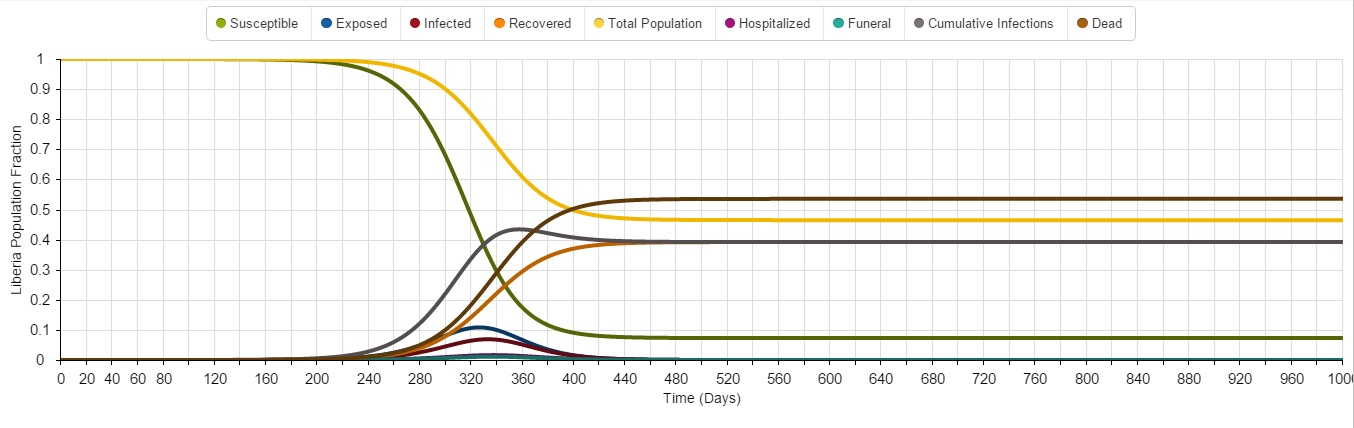
\includegraphics[width=0.7\textwidth]{LB_NoInt_SD_IM}
  \caption{ \bf Insight Maker results using the parameters of the first stage (Mar/14 to Sept/14) and assuming no intervention}
\label{fig:LB_IM_NoIn} 
\end{figure}\\

%Intervention 
\noindent As mentioned before, five parameters were calibrated for the second stage of the Ebola Outbreak, namely, community contact rate ($\beta_I$), hospital contact rate ($\beta_H$), funeral contact rate ($\beta_F$), time until hospitalization ($\gamma_H$) and probability a case is hospitalized ($\theta$). Figure \ref{fig:LB_IM_In} A. shows that there is not much change in the Total population and susceptible compartment, meaning that the virus was controlled;  Figure \ref{fig:LB_IM_In} B focuses on E, I, R, H , F and D compartments, showing that the international intervention causes a dramatic change in the behavior of such compartments.

\begin{figure}[!h]
  \centering
  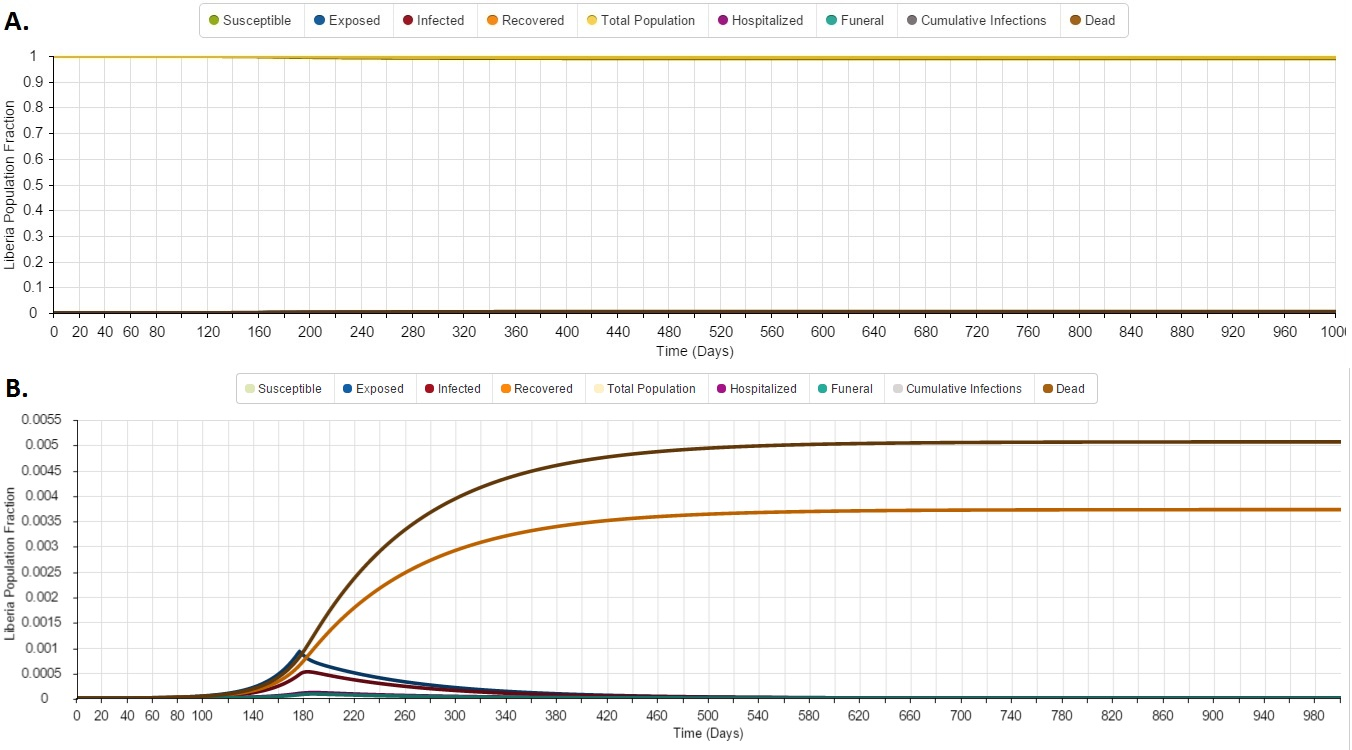
\includegraphics[width=0.7\textwidth]{LB_Int3_SD_IM}
  \caption{ \bf Insight Maker results using the parameters of the first stage (Mar/14 to Sept/14) and the second stage ( Sept/14 to Present)}
\label{fig:LB_IM_In} 
\end{figure}\\


%Comparing with WHO data

\noindent Finally, a comparison between the proposed model and World Health Organization data is shown in Figures \ref{fig:LB_IM_WHO} and \ref{fig:LB_IM_WHO2}. As depicted in \ref{fig:LB_IM_WHO} A and B there is a good fitting of our model with the data reported by WHO. Figure \ref{fig:LB_IM_WHO2} shows  the reported WHO data before and after intervention, the results of our model before and after intervention and the forecast for the coming months, predicting that after the system reaches an equilibrium, the proportion of deaths in Liberia product of the EVD would be 5.07\% approximately. 


\begin{figure}[!h]
  \centering
  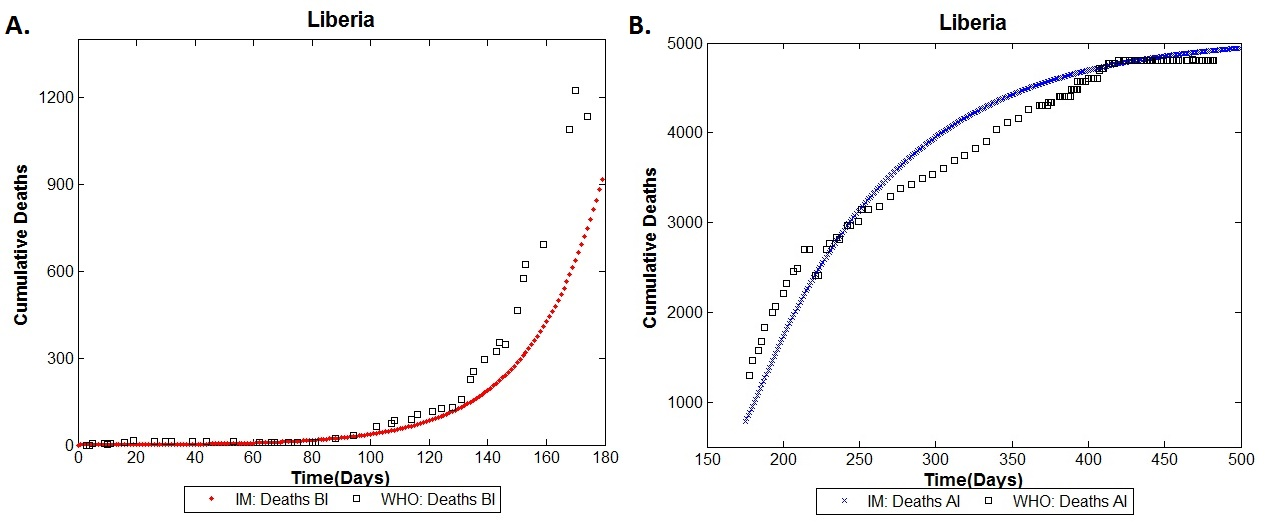
\includegraphics[width=0.7\textwidth]{LB_BI_AI_SD_WHO_IM}
  \caption{ \bf Comparison between World Health Organization (WHO) data and Insight Maker (IM) results using the parameters of A. the first stage (Mar/14 to Sept/14) and B. the second stage ( Sept/14 to July/15) for the cumulative deaths (D).}
\label{fig:LB_IM_WHO} 
\end{figure}\\



\begin{figure}[!h]
  \centering
  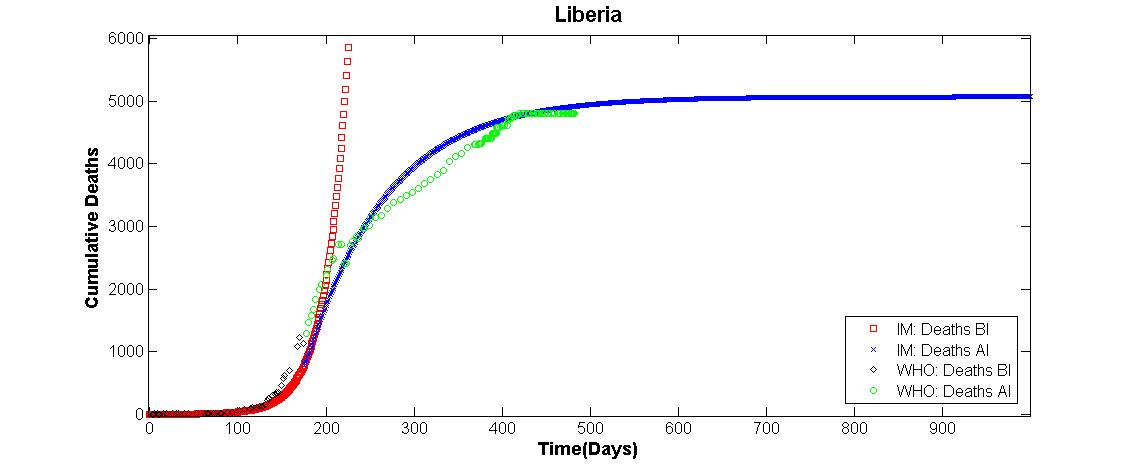
\includegraphics[width=0.7\textwidth]{LB_Int2_SD_WHO_IM}
  \caption{ \bf Comparison between World Health Organization (WHO) data and Insight Maker (IM) results using the parameters before intervention (BI) and after intervention (AI), for the cumulative deaths (D).}
\label{fig:LB_IM_WHO2} 
\end{figure}\\


%%MATHEMATICA DESCRIPTION
\newpage
\subsection{Mathematica}
We drew the plots in the previous section also with Mathematica, and got almost same result. One additional plot we draw in Mathematica is phase portrait of the system (Figure).

\begin{figure}[!h]
  \centering
  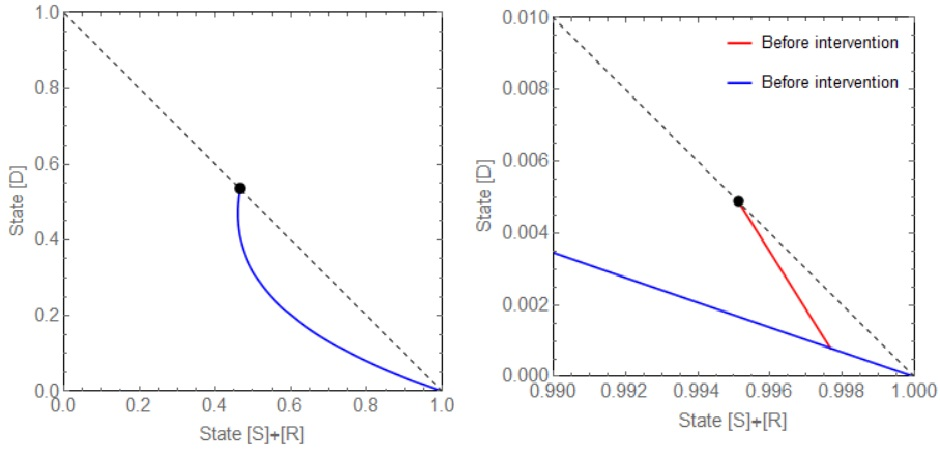
\includegraphics[width=0.7\textwidth]{PhasePortrait}
  \caption{Projection of phase portrait to (Susceptible + Recovered, Dead) space. (Blue) - without intervention, (Red) - with inter vention, (Dots) - where the phase converges (equilibrium).}
\label{fig:Phase Portrait}
\end{figure}



\end{document}
